\documentclass[border=3pt]{standalone}

% Tikz
\usepackage{tikz}
\usetikzlibrary{calc}

% Polar Coordinates
\newcommand{\drawpolar}[4]{\draw[thick] (#1,#2) -- ({#1+#3**cos(#4)}, {#2+#3**sin(#4)});}

\usepackage{amsmath, physics}

\begin{document}
	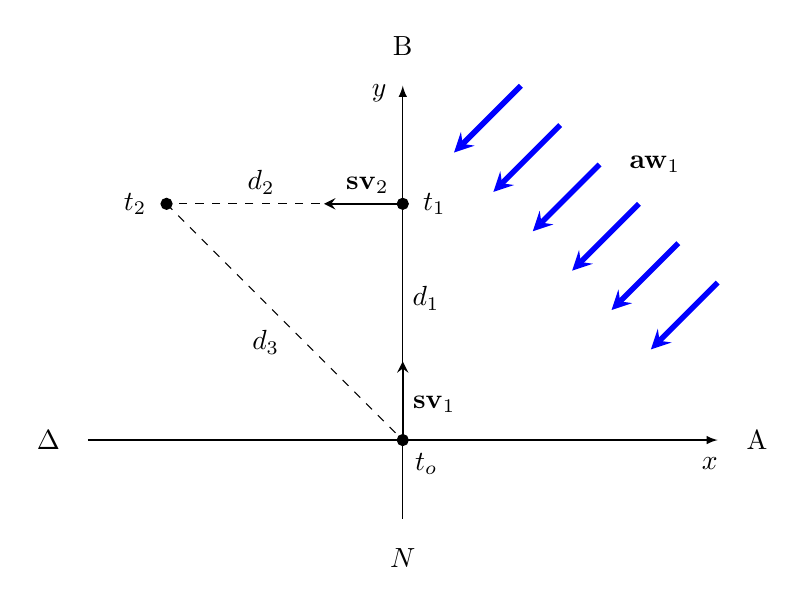
\begin{tikzpicture}
%		%Grid
%		\def\length{4}
%		\draw[thin, dotted] (-\length,-\length) grid (\length,\length);
%		\foreach \i in {1,...,\length}
%		{
%			\node at (\i,-2ex) {\i};
%			\node at (-\i,-2ex) {-\i};	
%		}
%		\foreach \i in {1,...,\length}
%		{
%			\node at (-2ex,\i) {\i};	
%			\node at (-2ex,-\i) {-\i};	
%		}
%		\node at (-2ex,-2ex) {0};
		
		%Coordinates
		\coordinate (A) at (0,0);
		\coordinate (B) at (0,3);
		\coordinate (C) at (-3,3);
		
		%Axis
		\draw[-latex] (-4,0) node[shift={(-0.5,0)}] {$\Delta$} -- (4,0) node[shift={(-0.1,-0.3)}] {$x$} node[shift={(0.5,0)}] {$\mathrm{A}$} ;
		\draw[-latex] (0,-1) node[shift={(0,-0.5)}] {$N$} -- (0,4.5) node[shift={(-0.3,-0.1)}] {$y$} node[shift={(0,0.5)}] {$\mathrm{B}$} ;
		
		%Ship
		\draw[draw=black, fill=black] (A) circle (2pt);
		\draw[draw=black, fill=black] (B) circle (2pt);			
		\draw[draw=black, fill=black] (C) circle (2pt);
		%%Velocities
		\draw[-stealth, thick] (A) -- +(0,1) node[pos=0.45, right] {$\vb{sv}_1$};
		\draw[-stealth, thick] (B) -- +(-1,0) node[pos=0.45, above] {$\vb{sv}_2$};
		%%Distance
		\draw[dashed] (C) -- (A) node[pos=0.42, shift={(0,-0.5)}] {$d_3$};
		\node[right] at ($(A)!0.6!(B)$) {$d_1$};
		\draw[dashed] (B) -- (C) node[pos=0.6, above] {$d_2$};
		
		%Wind
		\foreach \i in {1.5,2,...,4}
		{
			\draw[line width=2, -stealth, blue] (\i,-\i+6) -- ({1.2*cos(225)+\i},{1.2*sin(225)-\i+6});			
		}
		
		%Nodes
		\node[shift={(0.3,-0.3)}] at (A) {$t_o$};
		\node[shift={(+0.4,0)}] at (B) {$t_1$};
		\node[shift={(-0.4,0)}] at (C) {$t_2$};
		\node[shift={(-0.3,0)}] at (3.5,3.5) {$\vb{aw}_1$};
		
	\end{tikzpicture}
\end{document}
